% ======================================================================
% Sections 4 and 5: Study 1 (literature) and Study 2 (patents)
% Every number in this file is copied from raw_materials/experimental_log.md.
% ======================================================================

\section{Study 1: Literature Evidence}
\label{sec:study1}

Study~1 is the research line in which the structural-hole premise was first formulated. It covers the V5 literature corpus, the frozen V9 analysis of an AI-family $\times$ decision-family matrix, and the network lines V6--V11.1. We report it together with a data-validity re-analysis completed on 2026-11-18. Unless stated otherwise, the figures in this section are graded DIRECT. The network results in Section~\ref{sec:study1_network} are HISTORICAL / USER\_REPORTED and are labelled as such.

\subsection{Corpus, coding and test design}
\label{sec:study1_corpus}

The corpus comprises 2,118 source documents, of which 1,729 were parsed. Parsing yielded 26,501 candidate evidence records, of which 6,499 met the strict inclusion filter. An LLM pipeline assigned each evidence sentence to one of 10 AI families and one of 12 decision families. The result is a bipartite matrix of 120 cells. Deduplicating within each document gives 2,180 document-level edges. Of the 120 cells, 104 are observed. The 16 zero cells are disjoint from the 16 depleted cells reported below. Most edges (86.5\%) come from AI-track documents. For AI family $a$ and decision family $d$ with marginal degrees $k_a$ and $k_d$, the expected count is
\begin{equation}
E_{ad} = \frac{k_a\,k_d}{M}, \qquad M = 2{,}180 .
\label{eq:s1_expected}
\end{equation}

Each cell was evaluated with four tests:
\begin{enumerate}
  \item a fixed-degree stub Monte Carlo null ($R = 10{,}000$; seed 20260918);
  \item an exact hypergeometric test;
  \item a document-preserving within-document swap MCMC (5,000 samples, burn-in 43,600, thinning 4,360; seed 20260919);
  \item a raw-record exact test on the non-deduplicated records ($n = 3{,}125$).
\end{enumerate}
The Benjamini--Hochberg procedure controls the false discovery rate within the 120 cells \citep{benjamini1995controlling}. The frozen core rule requires three things: $q \le .05$ in the main, exact and document-preserving tests, the same direction in all three, and the raw test as well. Thirty-two cells meet this rule, 16 enriched and 16 depleted. ``Depleted'' and ``enriched'' are statistical descriptions relative to these nulls. They are not evidence of separation, and we do not call depleted cells gaps (Section~\ref{sec:design}).

\subsection{Direction and robustness of the depleted cells}
\label{sec:study1_direction}

Appendix~\ref{app:sens} lists the 16 depleted cells with their observed counts. The most extreme cell is \texttt{PREDICTION\_RISK\_ESTIMATION}~$\times$ \texttt{HUMAN\_REVIEW\_ACCOUNTABILITY}, with $O = 6$ against $E = 44.9$.

\paragraph{Computational robustness.} An independent re-implementation of the exact and raw tests reproduces the official $q$ values to within $|\Delta q| \le 6\times10^{-12}$. The Jaccard overlap of the 32-cell core is .94. Across 20 Monte Carlo seeds, 31 cells are in the core under every seed, including all 16 depleted cells. The 2 boundary cells are exactly the one-in / one-out pair identified by the human-corrected sidecar.

\paragraph{Compositional robustness.} Under a track-stratified null, which fixes the composition of AI-track and decision-track documents, 16/16 depleted and 16/16 enriched cells remain significant with unchanged direction. The dominance of AI-track documents therefore does not produce the pattern. Records from depleted core cells pass the strict filter more often than records from other cells (38\% vs 28\%). The depletion is therefore not created by the filter discarding records from these cells.

\paragraph{Temporal robustness.} Figure~\ref{fig:study1_direction} splits the documents into those from 2023 or earlier and those from 2024 or later. All 16 cells are depleted in both periods (16/16), and the change between periods does not differ from a permutation null ($p = .86$). Within this corpus the under-integration is persistent and shows no sign of closing.

\begin{figure}[t]
  \centering
  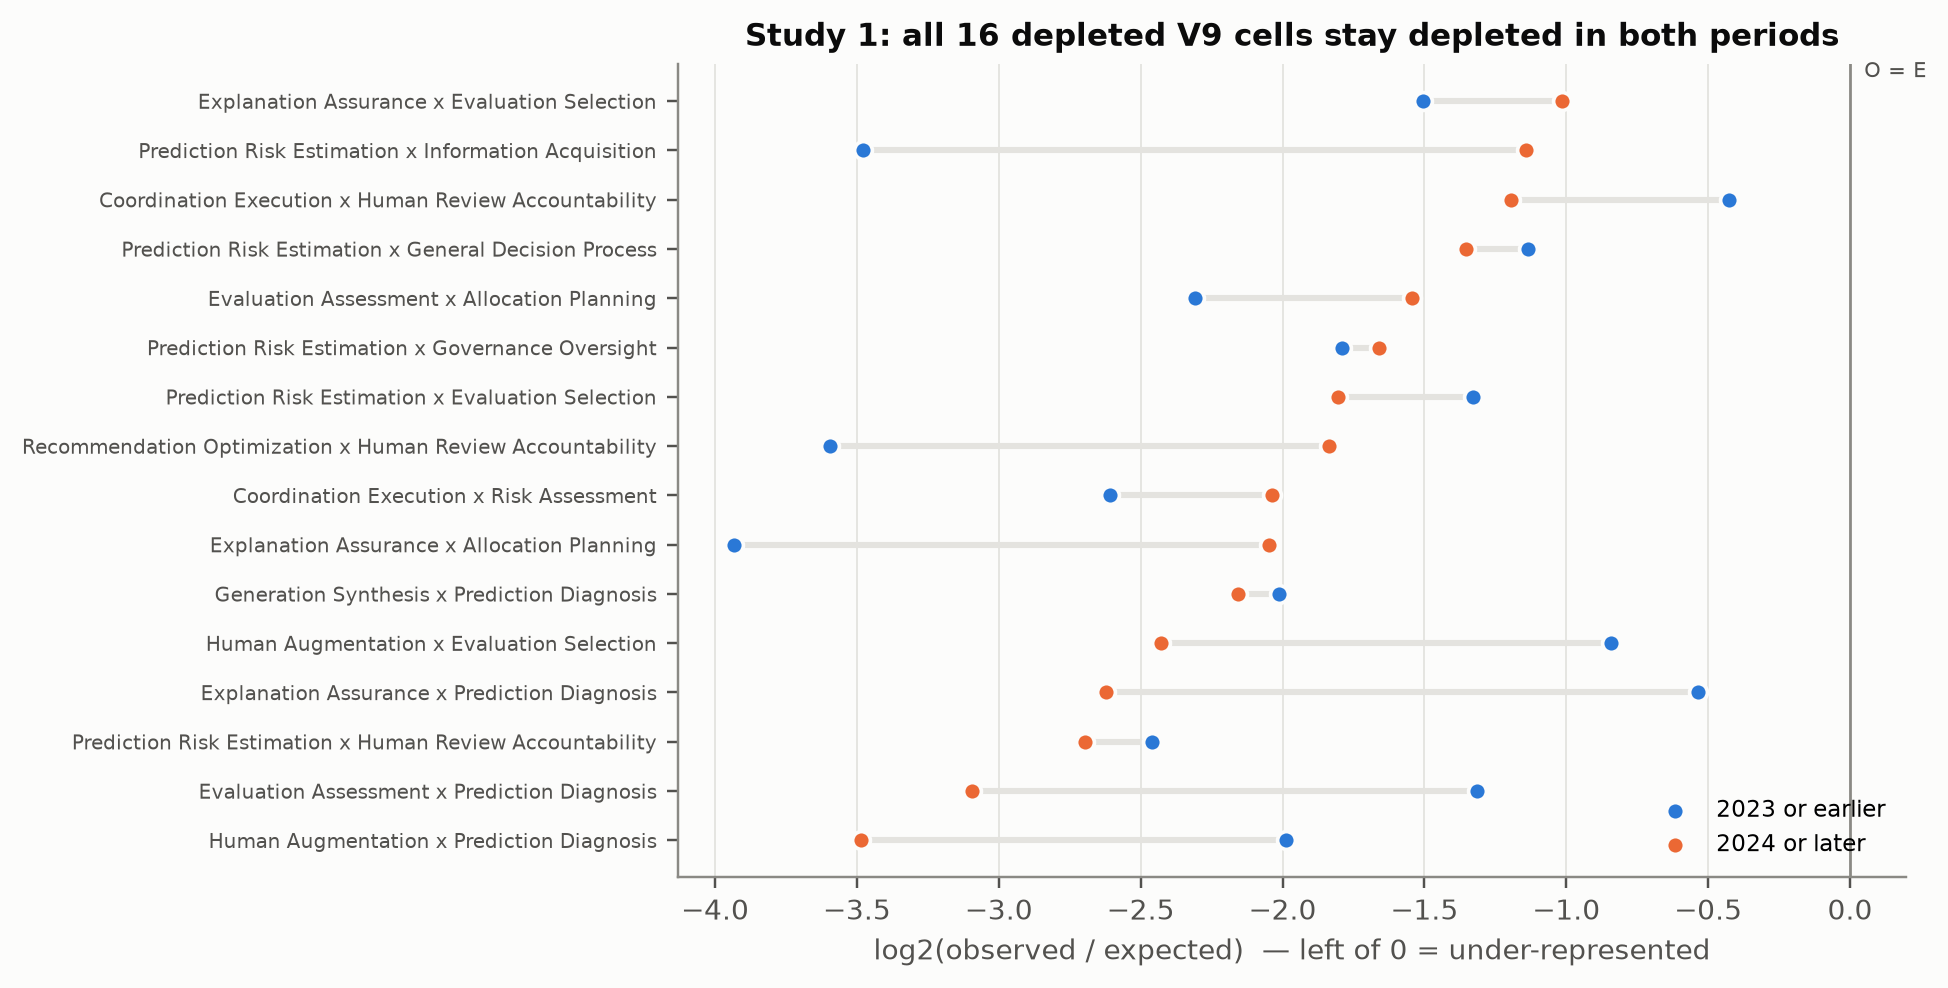
\includegraphics[width=\linewidth]{fig_study1_direction.png}
  \caption{Study~1: $\log_2(O/E)$ for each of the 16 depleted V9 cells, for documents from 2023 or earlier (blue) and 2024 or later (orange). The vertical line marks $O = E$. All 16 cells lie below $O = E$ in both periods (16/16), and the change between periods does not differ from a permutation null ($p = .86$). The direction is robust, but statistical significance does not survive realistic misclassification (Section~\ref{sec:study1_reliability}). These are depleted cells, not gaps. DIRECT.}
  \label{fig:study1_direction}
\end{figure}

\paragraph{Limits of triangulation.} The direction is less secure once the coding instrument changes:
\begin{itemize}
  \item Under keyword (stage-1) coding, 13/16 depleted cells keep the same direction.
  \item Same-term self-pairing inflates the strongest enriched cell (prediction $\times$ prediction). In that cell, 33\% of records pair the same term (e.g., ``forecasting'') on both sides. Removing these records drops 2 prediction-related depleted cells from the core.
  \item A rule-based keyword matrix removes 741 same-term records and leaves 1,431 document edges. In it, 13/16 depleted cells keep the same direction, 6 are significant and 0 are significantly reversed, but only 7 cells reach the four-test core.
\end{itemize}
The direction of the depletions is thus robust to seeds, source tracks and periods. The composition of the significant core, by contrast, depends on how sentences are coded. Appendix~\ref{app:sens} summarises all robustness checks.

\subsection{Measurement reliability and misclassification}
\label{sec:study1_reliability}

Table~\ref{tab:reliability} reports chance-corrected agreement (Cohen's $\kappa$; \citealp{cohen1960coefficient}) for the AI and decision labels.

\begin{table}[t]
  \centering
  \small
  \caption{Coding reliability of the Study~1 labels (Cohen's $\kappa$). Model-to-model agreement shows that a tool is reproducible. It is not human inter-rater reliability. DIRECT.}
  \label{tab:reliability}
  \begin{tabular}{p{0.62\linewidth}rr}
    \toprule
    Comparison & AI $\kappa$ & Decision $\kappa$ \\
    \midrule
    Human vs human ($n = 20$) & 0.05 & 0.14 \\
    Pipeline LLM (qwen) vs first human coder ($n = 50$) & 0.27 & 0.12 \\
    Pipeline LLM test--retest (143 sides) & 0.64 & 0.63 \\
    Theory-merged taxonomy (7$\times$6), human vs human & 0.08 & 0.16 \\
    Two Claude models, blind, codebook v2 (250 records): Sonnet vs Haiku$^{a}$ & 0.72 (0.87) & 0.56 (0.82) \\
    Claude (codebook v2) vs reconciled human answers ($n = 20$) & 0.45 & 0.70--0.76 \\
    Pipeline qwen vs reconciled human answers & 0.11 & 0.29 \\
    \bottomrule
  \end{tabular}

  \smallskip
  \raggedright\footnotesize $^{a}$In brackets: agreement among sides that both models coded.
\end{table}

Agreement between human coders is very low ($\kappa$ = 0.05 for AI labels and 0.14 for decision labels). A coarser, theory-merged 7$\times$6 taxonomy does not improve it (0.08 / 0.16). The pipeline is stable on retest (0.64 / 0.63), but its agreement with the first human coder (0.27 / 0.12) and with reconciled human answers (0.11 / 0.29) is weak. Two Claude models coding blind under a revised codebook agree more closely (0.72 / 0.56). This agreement shows that the procedure is reproducible. It is not evidence of human inter-rater reliability. The revised codebook also changes what is coded: under codebook v2, 42--64\% of evidence sentences state no explicit decision function, against a pipeline rate of 18\%. Only about 9\% of matrix records are reproduced in the same cell by both new coders.

\paragraph{Analytic bound.} Let $T$ be a cell's count under error-free coding, and let $e_{\mathrm{AI}}$ and $e_{\mathrm{Dec}}$ be the non-differential (random) error rates of the two labels. Then
\begin{equation}
\frac{O^{\mathrm{obs}}}{E} - 1 = (1 - e_{\mathrm{AI}})(1 - e_{\mathrm{Dec}})\left(\frac{T}{E} - 1\right).
\label{eq:attenuation}
\end{equation}
Because the accuracy product is at most one, random error can only attenuate a depletion. It cannot create one. This is why the direction of the depleted cells can be defended. The bound also limits what the magnitudes mean. For the most extreme cell, even the 95\% upper bound requires an accuracy product of at least 0.71, whereas the human audit implies a product of about 0.07. Under a purely random-error model the two figures cannot be reconciled. The observed magnitude should therefore not be read as the magnitude that human-coded data would show.

\paragraph{Simulation.} Table~\ref{tab:misclass} rebuilds the matrix and reruns the BH exact test under six misclassification scenarios. When either human coding is taken as the truth, the median number of depleted cells that remain significant is 0, although 11 and 12 cells keep their direction. Only the mildest error scenario (20\% random error) and the Claude-consensus scenario keep a non-zero median of significant cells (7 and 4). No scenario produced a spurious depleted cell.

\begin{table}[t]
  \centering
  \small
  \caption{Misclassification simulation for the 16 depleted cells: 300 runs per scenario. Each run rebuilds the matrix and reruns the BH exact test. Entries are the median (5th--95th percentile) number of cells. No scenario produced a spurious depleted cell. DIRECT.}
  \label{tab:misclass}
  \begin{tabular}{lll}
    \toprule
    Scenario & Still significant & Still depleted \\
    \midrule
    First human coder as truth & 0 (0--1) & 11 (8--13) \\
    Reconciled human as truth & 0 (0--1) & 12 (10--14) \\
    20\% random error + 20\% deletion & 7 (5--10) & 16 (15--16) \\
    40\% random error + 20\% deletion & 0 (0--1) & 14 (12--16) \\
    60\% random error + 20\% deletion & 0 (0--0) & 10 (7--13) \\
    Claude consensus (codebook v2) as truth & 4 (3--6) & 14 (12--15) \\
    \bottomrule
  \end{tabular}
\end{table}

The re-analysis of 2026-11-18 reached four verdicts:
\begin{itemize}
  \item directional under-integration is DEFENSIBLE;
  \item ``16 statistically robust depleted pairs'' is NOT DEFENSIBLE as measured;
  \item Burt structural hole: STOP, so the broker search is discontinued;
  \item a research gap is NOT SUPPORTED.
\end{itemize}

\subsection{Network lines V6--V11.1 and Gap Validity}
\label{sec:study1_network}

Successive versions of Study~1 searched citation, co-author and higher-order networks for Burt brokers (Table~\ref{tab:network_lines}). No line confirmed a broker. The V10.1 external review of 8 candidate pairs refuted 6 and left 2 unresolved. The V11.1 identity and peer validation rejected 3 of 4 candidates and found the evidence on the fourth insufficient.

\begin{table}[t]
  \centering
  \small
  \caption{Network search for Burt brokers, V6--V11.1. All rows are HISTORICAL / USER\_REPORTED. They are taken from earlier project logs or reported by the researcher, and the raw files were not re-verified.}
  \label{tab:network_lines}
  \setlength{\tabcolsep}{4pt}
  \begin{tabular}{l p{0.17\linewidth} p{0.33\linewidth} p{0.17\linewidth} l}
    \toprule
    Version & Line & Scale & Result & Grade \\
    \midrule
    V6 & citation SNA & 458 leads; 13 G2 candidates & 0 confirmed & HIST./USER \\
    V7 & author SNA & 446 works; 8 cross-domain authors; 2 focal candidates & 0 confirmed & HIST./USER \\
    V8 & citation enrichment & 1,111 citing works; 5,592 references & unconfirmed & HIST./USER \\
    V9 & citation line & 3,983 discovery + 3,897 confirmation works (7,880 total) & no confirmed Burt result & HIST./USER \\
    V10 & higher-order network & 14 exploratory candidates $\rightarrow$ 8 pairs / 7 brokers & exploratory only & HIST./USER \\
    V10.1 & external review & 8 candidate pairs & 6 refuted, 2 unresolved, 0 confirmed & HIST./USER \\
    V11 & co-author SNA & 26,443 V9 authors; 30,140 merged authors & 0 confirmed & HIST./USER \\
    V11.1 & external identity / peer validation & 95 OpenAlex requests; 7,880 works examined; 4 candidates & 3 rejected, 1 insufficient, 0 confirmed & HIST./USER \\
    \bottomrule
  \end{tabular}

  \smallskip
  \raggedright\footnotesize HIST./USER = HISTORICAL / USER\_REPORTED.
\end{table}

These lines could not have carried Burt's construct even with perfect data (Section~\ref{sec:theory}). A co-author network is a one-mode projection of author--work affiliation data \citep{newman2001scientific}, so a shared paper is not a directed flow between the two authors. Candidate screens based on centrality, such as the share of shortest paths through a node \citep{freeman1977set}, do not establish brokerage. Brokerage requires directed open two-paths between actors with group membership \citep{gould1989structures}, and Burt's benefits rest on non-redundant real contacts \citep{burt1992structural}.

The Gap Validity check (version V1, a DIRECT sidecar) makes the same point for the functional matrix itself. In the bipartite family network, all 16 depleted cells have alternative routes (16/16). The indirect term of Burt constraint is also identically zero in a strict bipartite graph. A depleted cell is therefore neither a disconnection nor a position whose constraint could reveal closure.

Study~1 therefore supports one claim only: the AI--decision pairs in this literature co-occur less often than their margins imply, and they do so persistently. It also documents why co-occurrence data cannot carry the Burt construct. Testing the premise requires directed flows, which Study~2 supplies.

% ======================================================================

\section{Study 2: Patent Evidence}
\label{sec:study2}

Study~2 tests the premise on directed knowledge flows: applicant citations between US utility patents, with examiner-assigned CPC classes as group labels. Four preregistrations, frozen in public commits before data access (aggregate test) or before computation (follow-ups), fixed definitions, null models, decision rules, sensitivity checks and stop rules \citep{nosek2018preregistration}: the aggregate test (\texttt{a8f3289}), the V9 battery (\texttt{a6266f7}), the full replication suite (\texttt{d641256}) and the firm null (\texttt{b59fc71}) (Section~\ref{sec:design}; Appendix~\ref{app:prereg}). All results in this section are DIRECT.

\subsection{Data and the aggregate test}
\label{sec:study2_aggregate}

\paragraph{Data.} We use the USPTO PatentsView \texttt{pvgpatdis} tables, downloaded on 2026-11-18 \citep{uspto2026patentsview}. They contain 8,512,829 utility patents granted 1976--2025 and 152,631,929 citation rows. Of these rows, 87,414,291 fall in scope (citing year 2010--2025), and 63,083,371 of those are applicant citations. Citations serve as a proxy for knowledge flows \citep{jaffe1993geographic}. Examiner-added citations may not reflect what inventors knew, so the primary specification uses applicant citations only \citep{alcacer2006patent}. Before 2013, PatentsView labels non-examiner citations ``cited by other''. The applicant-only specification therefore effectively covers citing years 2013--2025.

The groups use grant years 2010--2025:
\begin{itemize}
  \item AI (CPC \texttt{G06N}): 94,929 patents;
  \item DEC (\texttt{G06Q10/04}, forecasting and optimisation, plus \texttt{G06Q10/06}, resources, workflow, management and decision analysis): 37,501;
  \item BRIDGE (both): 5,316;
  \item other business-method patents (BIZ-OTHER; \texttt{G06Q} excluding \texttt{G06Q10}): 150,170.
\end{itemize}
Bridge patents are excluded from the cross counts.

\paragraph{Statistic.} Citations are stratified by $s = $ (citing grant year, cited grant year). In each stratum, $\mathrm{out}_A(s)$ is the number of citations made by group-$A$ patents, $\mathrm{in}_B(s)$ is the number received by group-$B$ patents, and $M(s)$ is the total. The time-stratified configuration expectation is
\begin{equation}
E(A\!\rightarrow\!B) = \sum_{s} \frac{\mathrm{out}_A(s)\,\mathrm{in}_B(s)}{M(s)} ,
\label{eq:patent_expected}
\end{equation}
and the symmetric intensity is
\begin{equation}
\mathrm{OE}(A,B) = \frac{O(A\!\rightarrow\!B) + O(B\!\rightarrow\!A)}{E(A\!\rightarrow\!B) + E(B\!\rightarrow\!A)} .
\label{eq:oe}
\end{equation}

\paragraph{Why the test is relative.} Citing is field-local, so cross-field OE is usually below 1 even between fields no one would call separated. An absolute criterion ``$\mathrm{OE} < 1$'' would flag almost any pair of fields. The synthetic calibration, run before the real data, shows this. With no hole, $\mathrm{OE} = 0.388$, well below 1, yet it lies above the synthetic reference lowest quartile (0.356), the ratio is 0.99 (0.79--1.21), and the test correctly returns \texttt{HOLE\_NOT\_SUPPORTED}. With 30\% suppression of cross-group citations (OE 0.275; ratio 0.66, 0.52--0.83) or 50\% suppression (OE 0.223; ratio 0.47), the test detects the hole. The preregistered hypotheses are therefore relative:
\begin{itemize}
  \item \textbf{H1a:} $\mathrm{OE}(\mathrm{AI},\mathrm{DEC})$ lies in the lowest quartile $Q_1$ of both $\{\mathrm{OE}(\mathrm{AI},X)\}$ and $\{\mathrm{OE}(\mathrm{DEC},X)\}$. The reference set is the 179 CPC main groups in \texttt{G06}, \texttt{G16} and \texttt{H04} with at least 2,000 patents.
  \item \textbf{H1b:} the ratio $\mathrm{OE}(\mathrm{AI},\mathrm{DEC}) / \mathrm{OE}(\mathrm{AI},\mathrm{BIZ\text{-}OTHER})$ is below 1, with an upper 95\% confidence bound below 1.
\end{itemize}

\paragraph{Results.} Under the primary specification, $O = 30{,}843$ and $E = 10{,}112$. This gives $\mathrm{OE}(\mathrm{AI},\mathrm{DEC}) = 3.05$ (95\% CI 2.94--3.17; Poisson cluster bootstrap over citing patents, 2,000 replicates). Both directions are over-represented: AI$\rightarrow$DEC has $O = 21{,}820$ and $E = 6{,}686$ (O/E 3.26), and DEC$\rightarrow$AI has $O = 9{,}023$ and $E = 3{,}426$ (O/E 2.63). H1a fails: OE(AI,DEC) exceeds 97.8\% of the OE(AI,$X$) values and 92.2\% of the OE(DEC,$X$) values, against lowest-quartile thresholds of 0.787 (AI side) and 0.502 (DEC side) and medians of 1.240 and 1.095. H1b fails: the ratio is 1.69 (95\% CI 1.60--1.77), although the comparison pair is itself over-connected ($\mathrm{OE}(\mathrm{AI},\mathrm{BIZ\text{-}OTHER}) = 1.809$). The preregistered verdict is \texttt{HOLE\_NOT\_SUPPORTED}.

All six preregistered sensitivity specifications agree with it (0/6 disagree; Table~\ref{tab:aggregate}, Figure~\ref{fig:patent_sensitivity}), so the verdict is not fragile. OE ranges from 2.59 (s2, DEC broadened to all of \texttt{G06Q10}) to 4.25 (s6, bridge patents counted on both sides).

\begin{table}[t]
  \centering
  \caption{Aggregate test: primary and six preregistered sensitivity specifications. ``Ratio vs BIZ'' is OE(AI,DEC)/OE(AI,BIZ-OTHER) with 95\% bootstrap CI. ``Percentile'' is the share of the 179 reference values OE(AI,$X$) / OE(DEC,$X$) that OE(AI,DEC) exceeds. DIRECT.}
  \label{tab:aggregate}
  \footnotesize
  \setlength{\tabcolsep}{4pt}
  \begin{tabular}{p{0.26\linewidth}rlll}
    \toprule
    Specification & OE(AI,DEC) & Ratio vs BIZ (95\% CI) & Percentile AI / DEC & Verdict \\
    \midrule
    primary & 3.05 & 1.69 (1.60--1.77) & 97.8\% / 92.2\% & NOT\_SUPPORTED \\
    s1 all citation categories & 3.00 & 1.65 (1.55--1.75) & 98.9\% / 92.7\% & NOT\_SUPPORTED \\
    s2 DEC = all \texttt{G06Q10} & 2.59 & 1.43 (1.38--1.49) & 95.5\% / 89.9\% & NOT\_SUPPORTED \\
    s3 AI broadened (+\texttt{G06F18}, \texttt{G06V10/70}) & 2.69 & 1.56 (1.50--1.63) & 94.4\% / 86.6\% & NOT\_SUPPORTED \\
    s4 inventive codes only & 3.00 & 1.62 (1.54--1.70) & 97.7\% / 94.5\% & NOT\_SUPPORTED \\
    s5 citing 2015+ & 3.04 & 1.69 (1.61--1.78) & 98.2\% / 92.9\% & NOT\_SUPPORTED \\
    s6 bridge patents on both sides & 4.25 & 2.35 (2.23--2.47) & 100\% / 99.4\% & NOT\_SUPPORTED \\
    \bottomrule
  \end{tabular}
\end{table}

\begin{figure}[t]
  \centering
  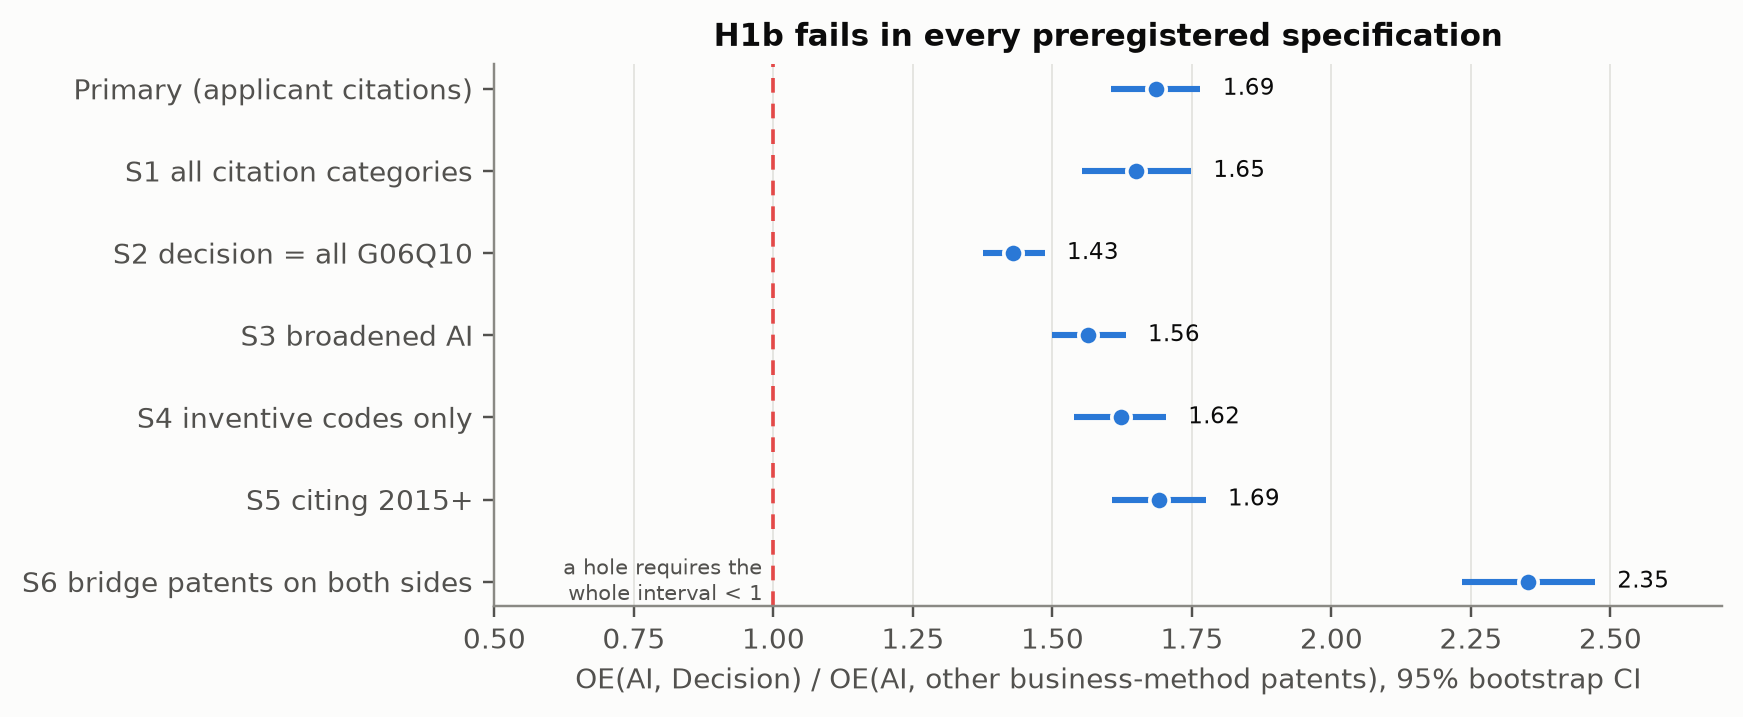
\includegraphics[width=\linewidth]{fig_patent_sensitivity.png}
  \caption{H1b ratio OE(AI,DEC)/OE(AI,BIZ-OTHER) for the primary and the six preregistered sensitivity specifications, with 95\% CIs (Poisson cluster bootstrap over citing patents, 2,000 replicates). A hole requires the whole interval to lie below the dashed line at 1. Every interval lies above 1, so H1b fails in all seven specifications. Table~\ref{tab:aggregate} gives the H1a percentiles.}
  \label{fig:patent_sensitivity}
\end{figure}

\paragraph{Trend (H2).} Figure~\ref{fig:patent_trend} plots OE(AI,DEC) by citing year. It falls from 3.90 in 2013 to 2.34 in 2025, with a weighted least-squares slope of $-0.097$ per year (95\% CI $-0.130$ to $-0.065$). The last-three-year OE is 2.69, against a reference median of 1.095, and the preregistered label is PERSISTENT. The over-connection is declining but remains more than twice the reference median. Appendix~\ref{app:sens} gives the yearly values.

\begin{figure}[t]
  \centering
  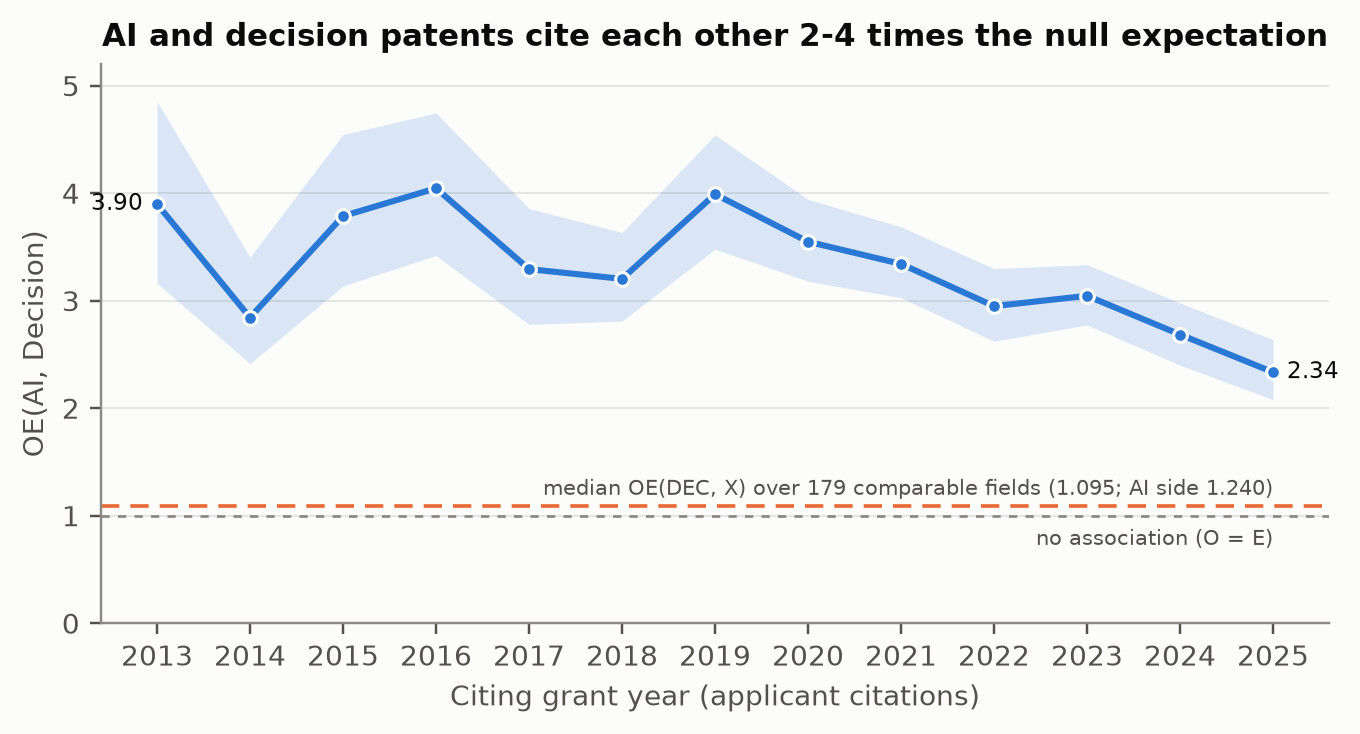
\includegraphics[width=\linewidth]{fig_patent_trend.png}
  \caption{OE(AI,DEC) by citing grant year, 2013--2025, with 95\% CI band. Applicant citations only; citing years begin in 2013 because PatentsView labels non-examiner citations ``cited by other'' before 2013. The dashed line is the median of the 179 comparable fields (1.095), and the dotted line is $O = E$. The last-three-year OE is 2.69. The preregistered label is PERSISTENT: OE declines but stays far above the reference median.}
  \label{fig:patent_trend}
\end{figure}

For RQ1, the evidence does not support a structural hole between AI and decision-making as knowledge domains, as operationalised here. AI and decision patents are over-connected relative to both reference sets. This is a failure to support a hole under a calibrated, preregistered test, not a proof that no separation exists under other operationalisations.

\subsection{The V9 battery on the CPC matrix and the M06-P null}
\label{sec:study2_cells}

Preregistration~2 ran the Study~1 battery on a patent analogue of the functional matrix. The matrix has 42 cells:
\begin{itemize}
  \item 6 AI-method rows: \texttt{G06N3} (neural), \texttt{G06N5} (knowledge-based), \texttt{G06N7} (probabilistic/fuzzy), \texttt{G06N10} (quantum), \texttt{G06N20} (machine learning) and \texttt{G06N\_OTHER};
  \item 7 decision-function columns: FORECAST\_OPTIMISE (\texttt{G06Q10/04}), RESOURCE\_SCHEDULING (\texttt{/0631}), WORKFLOW (\texttt{/0633}), RISK (\texttt{/0635}), STRATEGY (\texttt{/0637}), PERFORMANCE (\texttt{/0639}) and MGMT\_GENERAL (other \texttt{/06}).
\end{itemize}
The engine is a byte-identical copy of the V9 engine (SHA-256 \texttt{09c3d60c\ldots bc33}). The battery was run on three parts:
\begin{itemize}
  \item Part A, co-classification: 5,316 patents and 14,573 edges;
  \item Part B, applicant citations between AI-only and DEC-only patents: 30,843 citations and 66,056 edges;
  \item Part B with all citation categories: 38,252 citations and 80,849 edges.
\end{itemize}

\paragraph{A degenerate null and its replacement.} The preregistered document-preserving swap (M06) accepted 0 of 21,843,600 proposed swaps. The reason is structural: each patent contributes the complete row $\times$ column product of its codes, so every candidate swap targets an edge that already exists. The preregistered core is therefore empty by construction and carries no information about the data (amendment B1). Its replacement, M06-P, permutes column sets among documents within ($|$rows$|$, $|$cols$|$) strata, which preserves both margins and each document's block structure (5,000 samples). M06-P is a documented deviation from Preregistration~2 (amendment B1). It was itself frozen in Preregistration~3 (module P1) before it was computed.

\paragraph{Results.} The adapted full core contains 8 depleted and 7 enriched cells in Part A, 9 depleted and 8 enriched in Part B, and 8 and 8 in Part B with all categories. The numbers of $q \le .05$ cells by test (main / exact / raw / M06-P) are 20 / 20 / 29 / 22 in A and 22 / 22 / 27 / 25 in B \citep{benjamini1995controlling}. Table~\ref{tab:cells_both} lists the five cells depleted in both A and B and the four cells enriched in both under the three-test rule. Figure~\ref{fig:cpc_heatmap} shows the full matrices.

\begin{table}[t]
  \centering
  \small
  \caption{CPC cells that deviate in the same direction in co-classification (Part A) and citation flow (Part B). Values are O/E, with observed / expected counts in brackets. The adapted full core and three-test agreement give the same depleted set. \texttt{G06N10}~$\times$~PERFORMANCE is small-sample (expected count below 10 in B; 74 edges in the quantum row of A). Depleted cells, not gaps. DIRECT.}
  \label{tab:cells_both}
  \begin{tabular}{llll}
    \toprule
    AI method & Decision function & Part A & Part B \\
    \midrule
    \multicolumn{4}{l}{\emph{Depleted in both A and B}} \\
    \texttt{G06N3} & RISK & 0.78 (171 / 219.5) & 0.70 (1,050 / 1,510.6) \\
    \texttt{G06N5} & RISK & 0.87 (255 / 291.9) & 0.85 (2,008 / 2,366.6) \\
    \texttt{G06N3} & MGMT\_GENERAL & 0.87 (497 / 572.7) & 0.95 (4,189 / 4,414.8) \\
    \texttt{G06N20} & FORECAST\_OPTIMISE & 0.89 (994 / 1,120.9) & 0.93 (2,255 / 2,425.9) \\
    \texttt{G06N10} & PERFORMANCE & 0.08 (1 / 12.0) & 0 (0 / 8.9) \\
    \midrule
    \multicolumn{4}{l}{\emph{Enriched in both A and B (main + exact + raw)}} \\
    \texttt{G06N20} & RISK & 1.18 & 1.33 \\
    \texttt{G06N3} & FORECAST\_OPTIMISE & 1.09 & 1.17 \\
    \texttt{G06N5} & MGMT\_GENERAL & 1.16 & 1.06 \\
    \texttt{G06N7} & PERFORMANCE$^{a}$ & 1.15 & 1.16 \\
    \bottomrule
  \end{tabular}

  \smallskip
  \raggedright\footnotesize $^{a}$In the adapted full core only in Part B (Part A M06-P $q = .93$).
\end{table}

\begin{figure}[t]
  \centering
  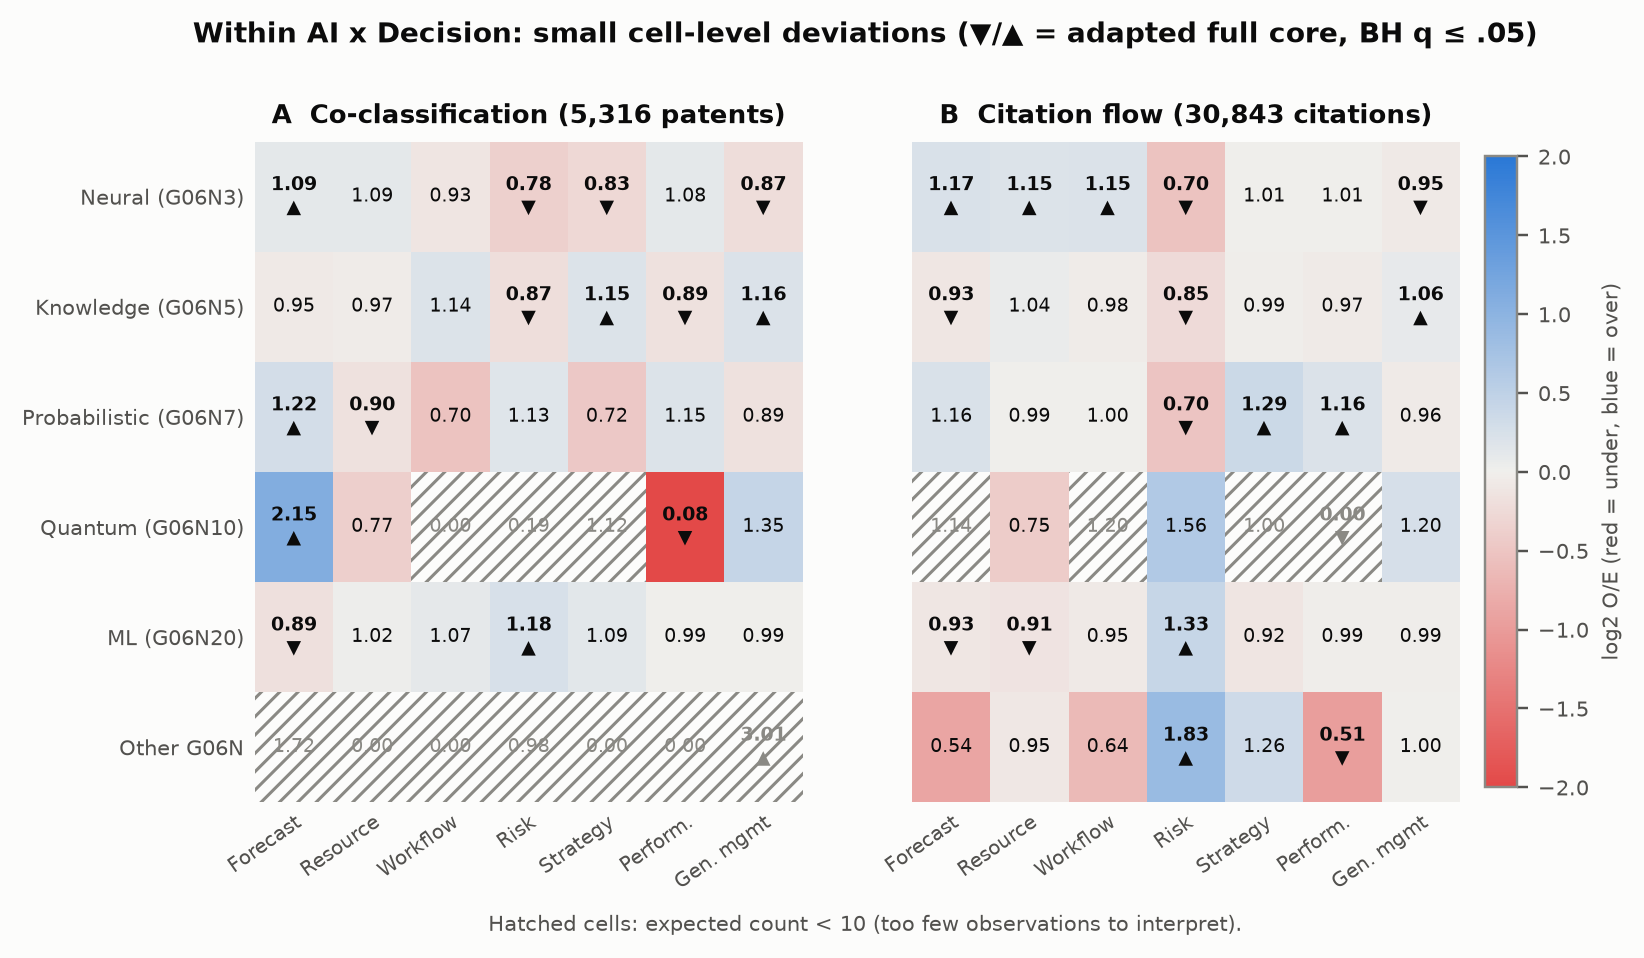
\includegraphics[width=\linewidth]{fig_cpc_heatmap.png}
  \caption{Cell-level $\log_2$ O/E in the 6$\times$7 CPC matrix: (A) co-classification, 5,316 patents; (B) applicant citation flow, 30,843 citations. Red marks under-representation and blue over-representation; hatched cells have expected count below 10. Triangles mark the adapted full core under M06-P (BH $q \le .05$): 8 depleted / 7 enriched in A and 9 / 8 in B. \texttt{G06N7}~$\times$~PERFORMANCE carries no marker in A because it is in the adapted full core only in B (Part A M06-P $q = .93$). No depleted cell replicates across the two time halves (Section~\ref{sec:study2_suite}).}
  \label{fig:cpc_heatmap}
\end{figure}

The magnitudes matter more than the counts. Apart from the quantum cell, the depleted O/E values in Table~\ref{tab:cells_both} lie between 0.70 and 0.95: modest shortfalls inside a domain pair whose overall intensity is about three times expectation. They are not separations, and we do not call them gaps. The quantum cell rests on 1 observed against 12.0 expected co-classifications and 0 against 8.9 expected citations; it is a small-sample result.

\subsection{Full replication suite}
\label{sec:study2_suite}

Preregistration~3 gives each original Study~1 research line a patent analogue on flow-valid data. Module P1 is the battery of Section~\ref{sec:study2_cells}; Table~\ref{tab:suite} maps P2--P10 to their original versions.

\begin{table}[t]
  \centering
  \small
  \caption{Full replication suite: patent analogues P2--P10 of the original Study~1 lines. DIRECT.}
  \label{tab:suite}
  \setlength{\tabcolsep}{4pt}
  \begin{tabular}{l p{0.19\linewidth} p{0.24\linewidth} p{0.40\linewidth}}
    \toprule
    Module & Original line & Patent analogue & Result \\
    \midrule
    P2 & V9.1 calibration & seeds, null false-positive rate, power, segmentation & A: 20 cells always $q \le .05$, 4 boundary; B: 22 always, 0 boundary. Mean false cells per null matrix 0.045 (A) / 0.049 (B). Power 67\% (A) / 79\% (B) \\
    P3 & V6/V8/V9 citation line & exploration/confirmation by time halves & A: 0 $\rightarrow$ 8 depleted; B: 3 $\rightarrow$ 11 depleted; 0 depleted cells replicate in both halves \\
    P4 & Study~1 human coding audit & title-keyword label face validity (pass if lift $\ge$ 1.5) & all 11 labels pass \\
    P5 & V7/V11 author SNA & firm citation network with Burt constraint & AI\_FIRM$\sim$DEC\_FIRM O/E 0.24; preregistered firm-level criterion met; MIXED median constraint 0.36 vs degree-matched null 0.444 ($p = .001$) \\
    P6 & V10.1 external review & removal falsification & 10/10 candidates refuted as indispensable; largest joint component 5,954 $\rightarrow$ 5,563 firms \\
    P7 & V10 higher-order network & co-assignment hyperedges & 2,546 hyperedges; 32\% join an AI\_FIRM with a DEC\_FIRM or MIXED firm \\
    P8 & V11.1 identity validation & alias check & 54 firms checked; 0 possible alias collisions \\
    P9 & Gap Validity V1 & indirect constraint term; alternative routes & indirect term 0 (bipartite); 20--30 alternative length-3 routes per depleted cell \\
    P10 & Limitation Scout & --- & NOT\_APPLICABLE (patents have no limitation section) \\
    \bottomrule
  \end{tabular}
\end{table}

\paragraph{P2: calibration.} The significant set is stable across seeds (20 $\times$ 10,000). On 1,000 stub-permutation null matrices (exact test with BH), the share of matrices with any false cell is 3.6\% (A) and 4.4\% (B). Power to detect a 20\% depletion in cells with $E \ge 100$ is 18/27 = 67\% in A and 23/29 = 79\% in B, so weaker or smaller depletions may be missed. Appendix~\ref{app:sens} reports the segmentation checks.

\paragraph{P3: replication across time.} The number of depleted cells rises from 0 (2010--2017) to 8 (2018--2025) in Part A and from 3 (2013--2018) to 11 (2019--2025) in Part B. No depleted cell replicates in both halves, in either part. Cell-level depletions in the patent data are therefore unstable over time, unlike the literature depletions of Section~\ref{sec:study1_direction}.

\paragraph{P4: label face validity.} Against other AI$\cup$DEC patents, all 11 labels pass the lift threshold of 1.5 on title-keyword hit rates; the lowest lift is 2.18 (\texttt{G06N20}; all lifts in Appendix~\ref{app:sens}). This check stands in for the Study~1 coding audit, but it is a title-keyword check, not a human audit.

\paragraph{P5: firm network.} Disambiguated assignees linked by applicant citations (self-citations excluded) form a network of 6,201 organisations with 20,681 ties and a total weight of 109,508 citations. Firms fall into three groups: 2,926 AI\_FIRM (only AI-only patents), 1,570 DEC\_FIRM and 1,705 MIXED. Group O/E is 0.24 for AI\_FIRM$\sim$DEC\_FIRM ($O = 886$, $E = 3{,}700$), 0.81 for AI\_FIRM$\sim$MIXED and 0.97 for DEC\_FIRM$\sim$MIXED. The preregistered firm-level hole criterion is met at this stage. Median Burt constraint \citep{burt1992structural} is 0.62 for AI\_FIRM, 0.76 for DEC\_FIRM and 0.36 for MIXED. Against a degree-matched label-permutation null, the MIXED median looks low (null median 0.444; one-sided $p = .001$). Read alone, this is the pattern the premise predicts, but it is not a confirmed structural hole: because it could arise mechanically from firms' portfolios, it motivated preregistration~4 (Section~\ref{sec:study2_firm}).

\paragraph{P6: removal falsification.} Ten MIXED firms with degree at least 5 had the lowest constraint. These candidates, later refuted as indispensable, were International Business Machines, General Electric, Tesla, ioCurrents, Google, Accenture, Amazon Technologies, T-Mobile USA, Optum Services and Strong Force VCN Portfolio 2019. After all 10 are removed, AI\_FIRM and DEC\_FIRM firms remain connected, and the largest component containing both groups shrinks only from 5,954 to 5,563 firms: 10/10 candidates are refuted as indispensable brokers. The suite's cross-weight-retained metric is identically 1 by construction and therefore uninformative; we draw no inference from it.

\paragraph{P7--P10.} Of 2,546 co-assignment hyperedges, 32\% join an AI\_FIRM with a DEC\_FIRM or MIXED firm (P7). The alias check found 0 possible collisions among 54 firms (P8). Gap Validity (P9) repeats the Study~1 finding: the indirect constraint term is 0 in the bipartite matrix, and every depleted cell has 20--30 alternative length-3 routes. The Limitation Scout (P10) does not apply to patents.

\subsection{Portfolio-preserving firm null}
\label{sec:study2_firm}

The P5 pattern could be mechanical. MIXED firms own both kinds of patents, and patents cite mainly within their own field, so specialist firms in different fields would cite one another rarely even if no firm brokered anything. Preregistration~4 therefore permutes the owner sets of patents within strata, keeping every firm's portfolio and group and the whole patent-level citation network fixed.
\begin{itemize}
  \item The primary strata are patent type $\times$ grant year (48 strata).
  \item The S-tech strata add technology mix: type $\times$ year $\times$ AI rows $\times$ DEC columns (1,795 strata).
\end{itemize}
Each null has 1,000 replicates, and replicate $r$ of scheme $s$ uses the seed sequence [20261119, $s$, $r$]. The scope is 127,114 patents, 14,600 firms and 162,339 citations. The identity permutation reproduces P5 exactly.

\begin{table}[t]
  \centering
  \small
  \caption{Portfolio-preserving firm null: 1,000 replicates per stratification, with one-sided lower-tail $p$ values. T1 is the O/E of ties between specialist AI and decision firms, and T2 is the median Burt constraint of MIXED firms. The verdict is PARTIAL in both stratifications. DIRECT.}
  \label{tab:firm_null}
  \footnotesize
  \setlength{\tabcolsep}{4pt}
  \begin{tabular}{p{0.22\linewidth}rlrlr}
    \toprule
    & & \multicolumn{2}{c}{Primary (type $\times$ year)} & \multicolumn{2}{c}{S-tech (+ technology mix)} \\
    Statistic & Observed & Null median [95\%] & $p$ & Null median [95\%] & $p$ \\
    \midrule
    T1 OE(AI\_FIRM$\sim$DEC\_FIRM) & 0.240 & 0.356 [0.317--0.398] & .001 & 0.307 [0.277--0.345] & .001 \\
    T2 MIXED median constraint & 0.358 & 0.104 [0.098--0.111] & 1.000 & 0.116 [0.110--0.122] & 1.000 \\
    OE AI\_FIRM$\sim$MIXED & 0.809 & 1.000 & .001 & 0.985 & .001 \\
    OE DEC\_FIRM$\sim$MIXED & 0.970 & 1.009 & .001 & 1.025 & .001 \\
    \bottomrule
  \end{tabular}
\end{table}

\paragraph{Results.} Table~\ref{tab:firm_null} and Figure~\ref{fig:firm_null} report the results. The observed specialist O/E (T1 = 0.240) lies below every null replicate ($p = .001$, the smallest value attainable with 1,000 replicates). The null medians are much lower than 1: 0.356 under the primary and 0.307 under the S-tech stratification. Portfolio composition alone thus produces most of the separation between specialist firms. Of the observed shortfall of T1 below $O = E$, the null reproduces 85\% under the primary stratification and 91\% under S-tech. The remainder is a residual specialist separation that the null does not explain. We report it as unexplained, not as a structural hole.

The brokerage reading of P5 does not survive. The observed MIXED median constraint (0.358) lies above every null replicate (null medians 0.104 and 0.116; $p = 1.000$). Real firms are more clustered than the portfolio null implies, and mixed-portfolio firms show no brokerage advantage \citep{burt1992structural, burt2004structural}. The verdict is PARTIAL in both stratifications, so it does not depend on technology mix.

\begin{figure}[t]
  \centering
  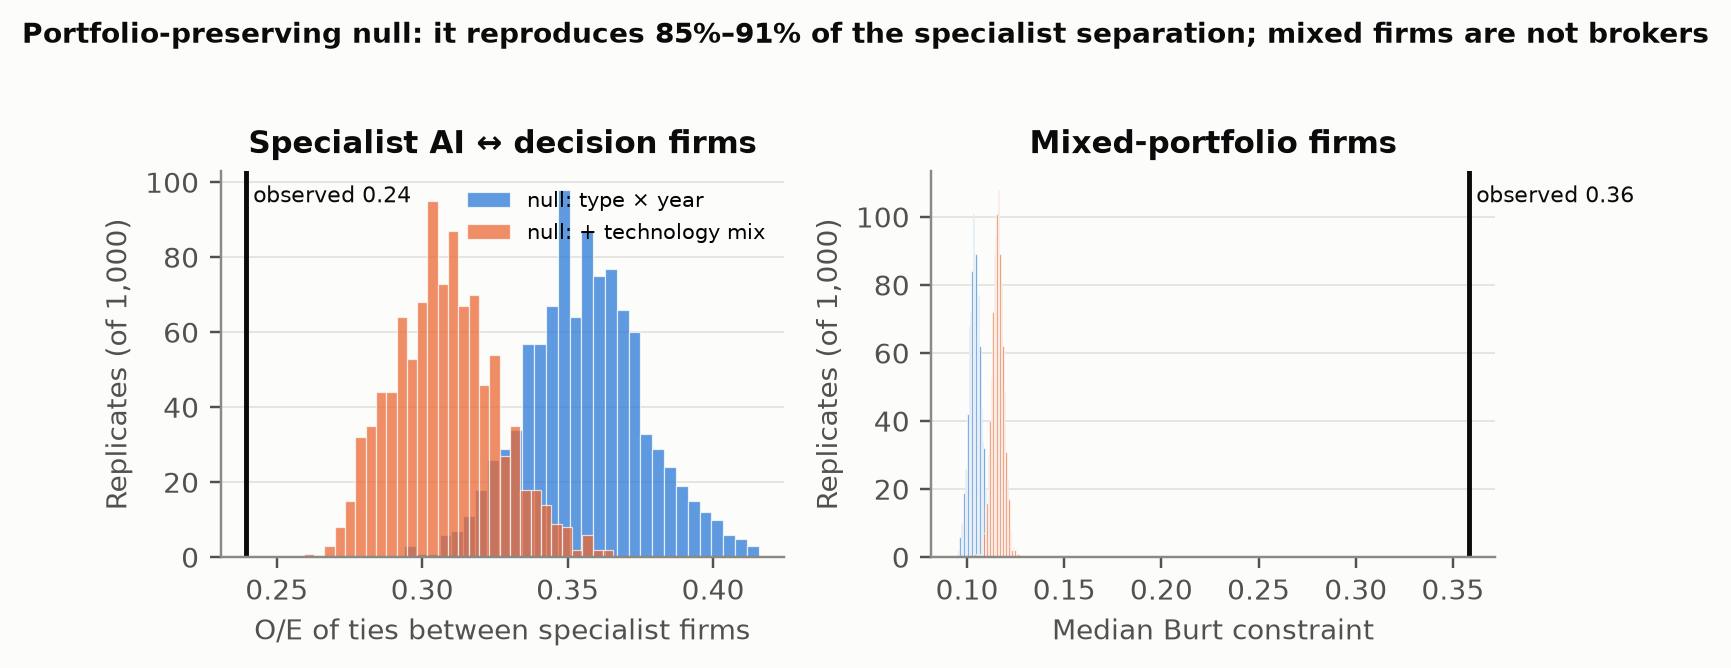
\includegraphics[width=\linewidth]{fig_firm_null.png}
  \caption{Portfolio-preserving firm null: 1,000 replicates under the primary (type $\times$ year; blue) and S-tech (+ technology mix; orange) stratifications. Every firm's portfolio and group and the patent-level citation network are held fixed. Left: O/E of AI\_FIRM--DEC\_FIRM ties, observed 0.240 against null medians of 0.356 and 0.307 ($p = .001$ each); the null reproduces 85\% and 91\% of the specialist separation. Right: MIXED median Burt constraint, observed 0.358 against null medians of 0.104 and 0.116 ($p = 1.000$ each); mixed firms show no brokerage advantage. Verdict: PARTIAL in both stratifications.}
  \label{fig:firm_null}
\end{figure}

The contrast with P5 is the methodological point. Against a degree-matched label-permutation null, MIXED constraint looked low ($p = .001$). Against a null that preserves portfolios, it is high. The choice of null therefore determines the brokerage conclusion, and only the portfolio-preserving null holds fixed the structure that generates the data (Section~\ref{sec:discussion}). Because the null was frozen before computation \citep{nosek2018preregistration}, this reversal is not the product of choosing a null after seeing the results.

For RQ2, the evidence does not support a firm-level structural hole beyond what firms' technology portfolios mechanically imply. Specialist AI and decision firms are separated, but 85--91\% of that separation is reproduced by portfolio composition. Mixed-portfolio firms, the natural candidates for brokers, are more constrained than the null, not less.
